\documentclass[conference]{IEEEtran}
\IEEEoverridecommandlockouts
% The preceding line is only needed to identify funding in the first footnote. If that is unneeded, please comment it out.
\usepackage{cite}
\usepackage{amsmath,amssymb,amsfonts}
\usepackage{algorithmic}
\usepackage{graphicx}
\usepackage{textcomp}
\usepackage{subcaption}
\def\BibTeX{{\rm B\kern-.05em{\sc i\kern-.025em b}\kern-.08em
    T\kern-.1667em\lower.7ex\hbox{E}\kern-.125emX}}
\begin{document}

\title{User-Friendly IoT Data Management Framework}

\author{\IEEEauthorblockN{Hyun Bin Lee, Aravind Sagar, Zicheng Li}

\IEEEauthorblockA{ %\textit{Department of Computer Science} \\
\textit{University of Illinois at Urbana-Champaign}\\
Urbana, United States \\
\{lee559,asagar3,zli135\}@illinois.edu}
%\and
%\IEEEauthorblockN{Aravind Sagar}
%\IEEEauthorblockA{\textit{Department of Computer Science} \\
%\textit{University of Illinois Urbana-Champaign}\\
%Urbana, United States \\
%asagar3@illinois.edu}
%\and
%\IEEEauthorblockN{Zicheng Li}
%\IEEEauthorblockA{\textit{Department of Electrical and Computer Engineering} \\
%\textit{University of Illinois Urbana-Champaign}\\
%Urbana, United States \\
%zli135@illinois.edu}
}

\maketitle

%TODO write abstract
\begin{abstract}
We propose an extension framework of Hashemi et al.'s \cite{campbell} IoT Blockchain data sharing model. While this data sharing model guarantees transparency of data sharing, users cannot confidently make a coherent decision without effectively summarizing information provided by multiple parties. We introduce a user interface for people who are willing to share data collected by IoT devices. We envision most data requests come from IoT applications as these applications potentially need access to user data to improve quality of service. Our solution assists users by providing sufficient background information to decide whether he or she should grant/deny data requests from IoT applications or explicit data requests via Messaging Service introduced in the model. Our solution is composed of i) a front-end Android application that provides an efficient summary of each data object and data request and ii) a back-end server, hosted by third-party cloud service providers, that automates communication processes among Data Owner, Data Sources and Data Requesters. Our user study shows that our user-friendly framework provides sufficient information (by whom the data was requested and which sources collected the data) and guides end-users to make autonomous decisions on potentially sensitive data.
\end{abstract}

\section{Introduction}
Smaller and more power efficient processors enables almost everything in our life to collect information and access internet. This gave rise to the idea of “Internet of Things” (IoT). 
As IoT devices prevail, our society faces many new challenges. How do we store the vast amount of data generated by these devices? How do we manage and secure them? And, most importantly, how can we help the data owners to protect their privacy? Many research efforts have been made to address the first two challenges. Among them, Sayed Hadi Hashemi has introduced a framework that allows scalable and secure manipulation of IoT data in his paper “World of Empowered IoT Devices”. However, few have been done to address the last challenge. In this paper, we further improve Sayed’s framework by introducing an intuitive way, in the form of a user interface, for the user to categorize and define access-control policies to his/her data. In addition, we see the trend of processing IoT data on cloud, we add SGX support to the framework to enforce data security in cloud computing environment.

Our main contributions include:
\begin{enumerate}
	\item While most systems tag user data from the stand point of the developers, we give users the means to tag data in a way that is intuitive to them. This, combined with an easy-to use user interface, bring the security features to an accessible level to ordinary users.

	\item By adding SGX support, we made the existing framework resilient to security concerns when using an untrusted cloud service platform.
\end{enumerate}


\begin{figure}[t]
	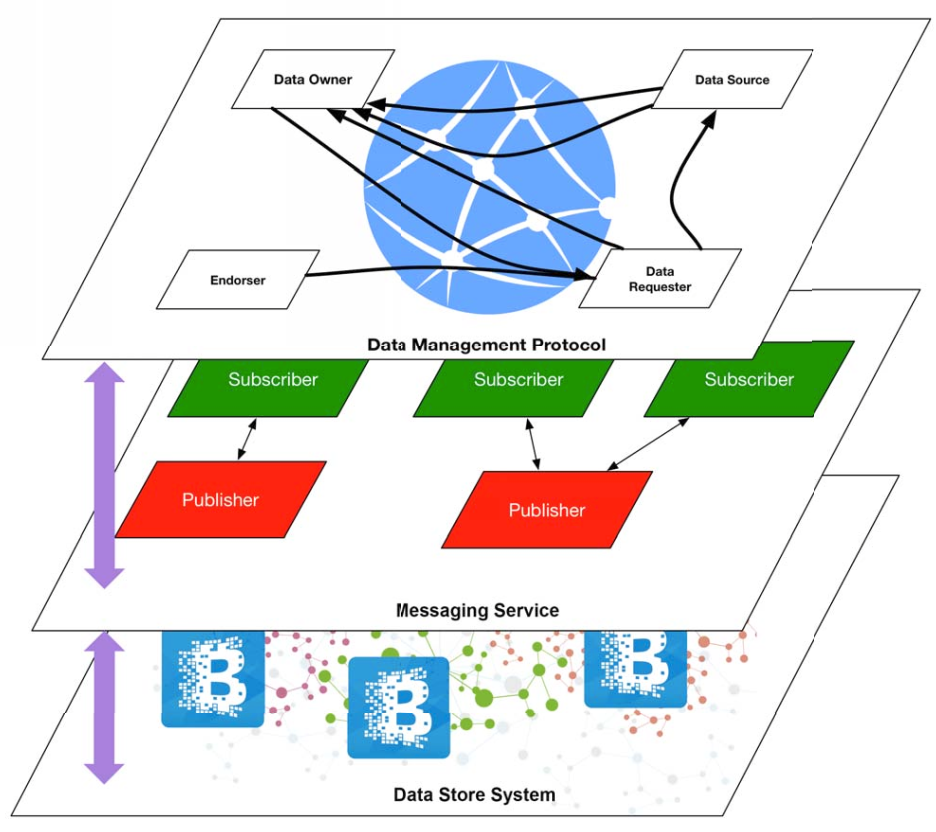
\includegraphics[width=0.95\linewidth]{campbell_framework.png}
	\caption{Structure of the a privacy-aware IoT framework}
	\label{fig:framework_campbell}
\end{figure}

\section{Background}
\subsection{Internet of Things}
The term Internet of Things (IoT) originated more than 15 years ago, when it was used to describe the work of the Auto-ID Labs at the
Massachusetts Institute of Technology (MIT) on networked radio-frequency identification (RFID) infrastructures~\cite{atzori}. The definition has since expanded to beyond the scopr of RFID technologies. A lot of modern definitions have been proposed, one of them being ``a global infrastructure for the Information Society, enabling advanced services by interconnecting (physical and virtual) things based on existing and evolving interoperable information and communication technologies''~\cite{itu}.

The applications of IoT are diverse, ranging from smart industries to smart homes. In smart home area, thermostats, security systems, and energy management systems are particularly growing fast. In this paper, we focus on IoT technologies related to individual users, and these mostly fall under the smart home category, though the general principles are applicable in all areas of IoT.

Recent years have seen a rapid growth of smart devices available commercially. Ecosystems like Samsung SmartThings, Google Home and Apple Homekit are competing to become the primary player in personal IoT devices space, and for good reason -  it is estimated that IoT could grow into a market worth \$7.1 trillion by 2020~\cite{idc}.

However, the rapid expansion of IoT market also means that many issues have been overlooked, and still need resolution. Some of the relevant issues are presented in `Related Works'.

\subsection{Security and privacy in IoT (Blockchain paper)}
IoT data security is crucial in protecting user privacy. In the paper ``World of Empowered IoT Devices" \cite{campbell}, a IoT data management system is proposed. This provides a user-centric, scalable, distributed and privacy-aware system to share data between the users (data owners) and third party data requesters.

In the data management protocol of this framework, user data is stored in trusted third-party entities, known as “data sources”. IoT users are known as “data owners” to the data their devices collected. Entities who are trying to get access to user data are known as “data requesters”. 

The data owner is the only party who can grant data requesters the right, called “capability”, to access its proprietary data. When the data requester needs data access, it contacts the data owner for the capability. After acquiring the capability, the data requester will access data at data source. Throughout the process, the data owner has the control its data.

To ensure data transparency, all data transactions are recorded using BlockChains. After a successful data transaction, the data server broadcasts the transaction and the publishers update their BlockChain Record. 

\subsection{Related Works}
Davies et. al. points out that privacy concerns could be a major factor preventing wide-spread adoption of IoT devices~\cite{davies}. Over-centralization of IoT systems is identified as a critical obstacle to eliminating concern over privacy. They propose a privacy mediator which sits in between IoT devices/data and outside world, and validates permissions according to the access control policies before any data is sent out. This model includes a trusted `cloudlet', which could be a local hub or a trusted server at the edge of the cloud. They also emphasize some important characteristics that a privacy-aware IoT system should have, like exposing summarized data, user anonymity, control over inferred sensors, and ease of use. However, the model's limitation is that data storage has to happen in the sensor or the cloudlet - this could be limiting when the number of sensors increase. The model also does not discuss any framework for how to identify legitimate third party applications, and how to make sure that the request originates from the same application as it is claiming to be from.

Data mining and clustering of IoT related articles expose major problem areas in IoT~\cite{zhang}. App over-privilege, environment mistrust, LAN mistrust and weak authentication are identified as some of the problem areas that needs work. They also conclude that permissioning needs to be more fine-grained, and recommend better standards and widely-applicable systems.

Security analysis of existing IoT systems show that serious vulnerabilities exist currently~\cite{smartthings}. An analysis of Samsung Smartthings ecosystem in particular, shows that apps in the ecosystem are overpriveleged, and vulnerabilities like event spoofing can lead to privacy violation and even more serious consequences like loss of property. This goes even further in showing that a centralized proprietary system is probably not the right way to deal with IoT.


\begin{figure}[t]
	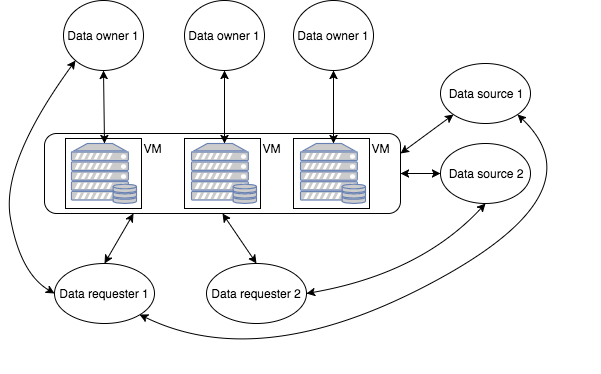
\includegraphics[width=0.95\linewidth]{mid_sem_graphic.png}
	\caption{Structure of the prototype framework}
	\label{fig:framework}
\end{figure}

\section{Problem and solution}
As evident from the previous sections, effectively addressing privacy concerns about the data generated by IoT devices is essential for the success of IoT. There are some proposed architectures which tackles this problem using user-oriented and decentralized systems. However, there's a lack of a user-facing component in such systems, which can effectively make the complex architectures usable to everyone. Our work is aimed at tackling this problem, which is "to build a user-facing component for a privacy-aware distributed user-centric IoT system (such as the blockchain based system described in \cite{campbell}), which improves the user friendliness of the system while maintaining strong security and privacy guarantees."

To accomplish this, we build the user-facing component for the blockchain based IoT architecture described in "World of empowerd IoT users \cite{campbell}". Since that system is still in development, we concentrate on the user facing components of the system, and simulate some of the external components.

The proposed work consists of 2 components:

\begin{enumerate}
	\item A smartphone app to manage IoT devices and data: Smartphones are becoming the preferred devices for internet access \cite{statcount}. Hence we build a smartphone app with which users can manage their IoT devices and data. The functionality provided by the app includes:

	\begin{enumerate}
		\item A centralized view of IoT generated data owned by them.

		\item A detailed view including the data source, access permissions and other details of this data.

		\item Permission request notifications from data requesters, and a way to accept or deny them.

		\item View, add, remove trusted parties.
	\end{enumerate}

	This is not a comprehensive list of the functionality, as we expect to add more as the project progresses. It also hides away some complexity from the users, like managing secure connection with the server described below, and managing user's private key etc. We also focus on the user-friendliness of the app, and expect to conduct user-research to find out what capabilities do users expect to find in such an app.
	
	\item A trusted server which manages the access control: This is the component which actually manages access control and capability issuance in accordance to the user's wishes. This is similar to cloudlets described in \cite{davies}, but with some key differences. First, we intend to leverage hardware technologies like Intel SGX to ensure that the server application can run on untrusted hosts. Second, this app does not store data within it; it simply interacts with the data owner, data sources and data requesters in accordance to the protocol outlined in \cite{campbell}.

	

\end{enumerate}

\section{Threat Model}
1. cellphone Trusted (we can use TrustZone based solution to be orthogonal to our solution)

2. data source Trusted

3. Endorser Trusted

4. data requesters NOT trusted

5. cloud NOT trusted

6. we are not responsible for user misassigning policies. instead we aim to minimize it

\begin{figure*}[t]
	\begin{subfigure}{0.24\textwidth}
	\frame{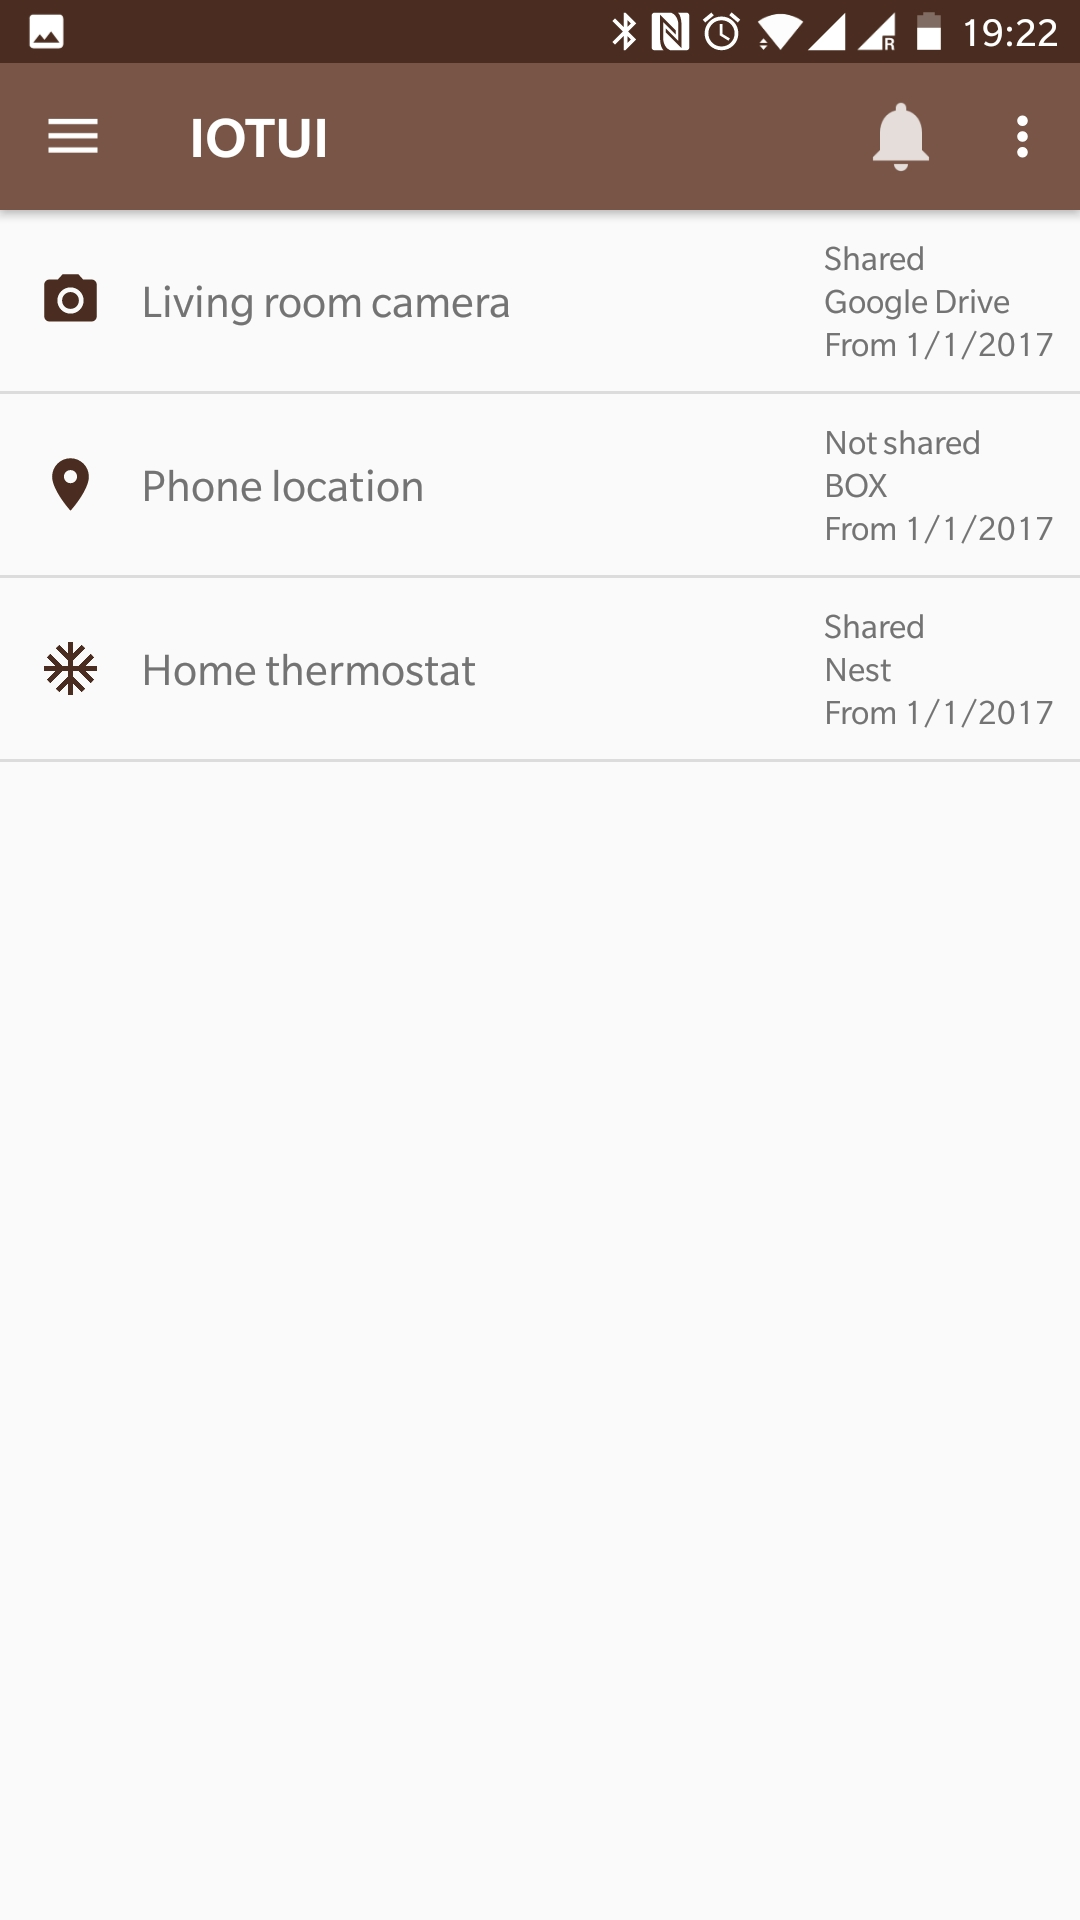
\includegraphics[width=0.95\linewidth]{screen1.jpg}}
	\caption{Overview of user's data}
	\label{fig:screen1}
	\end{subfigure}
	\begin{subfigure}{0.24\textwidth}
	\frame{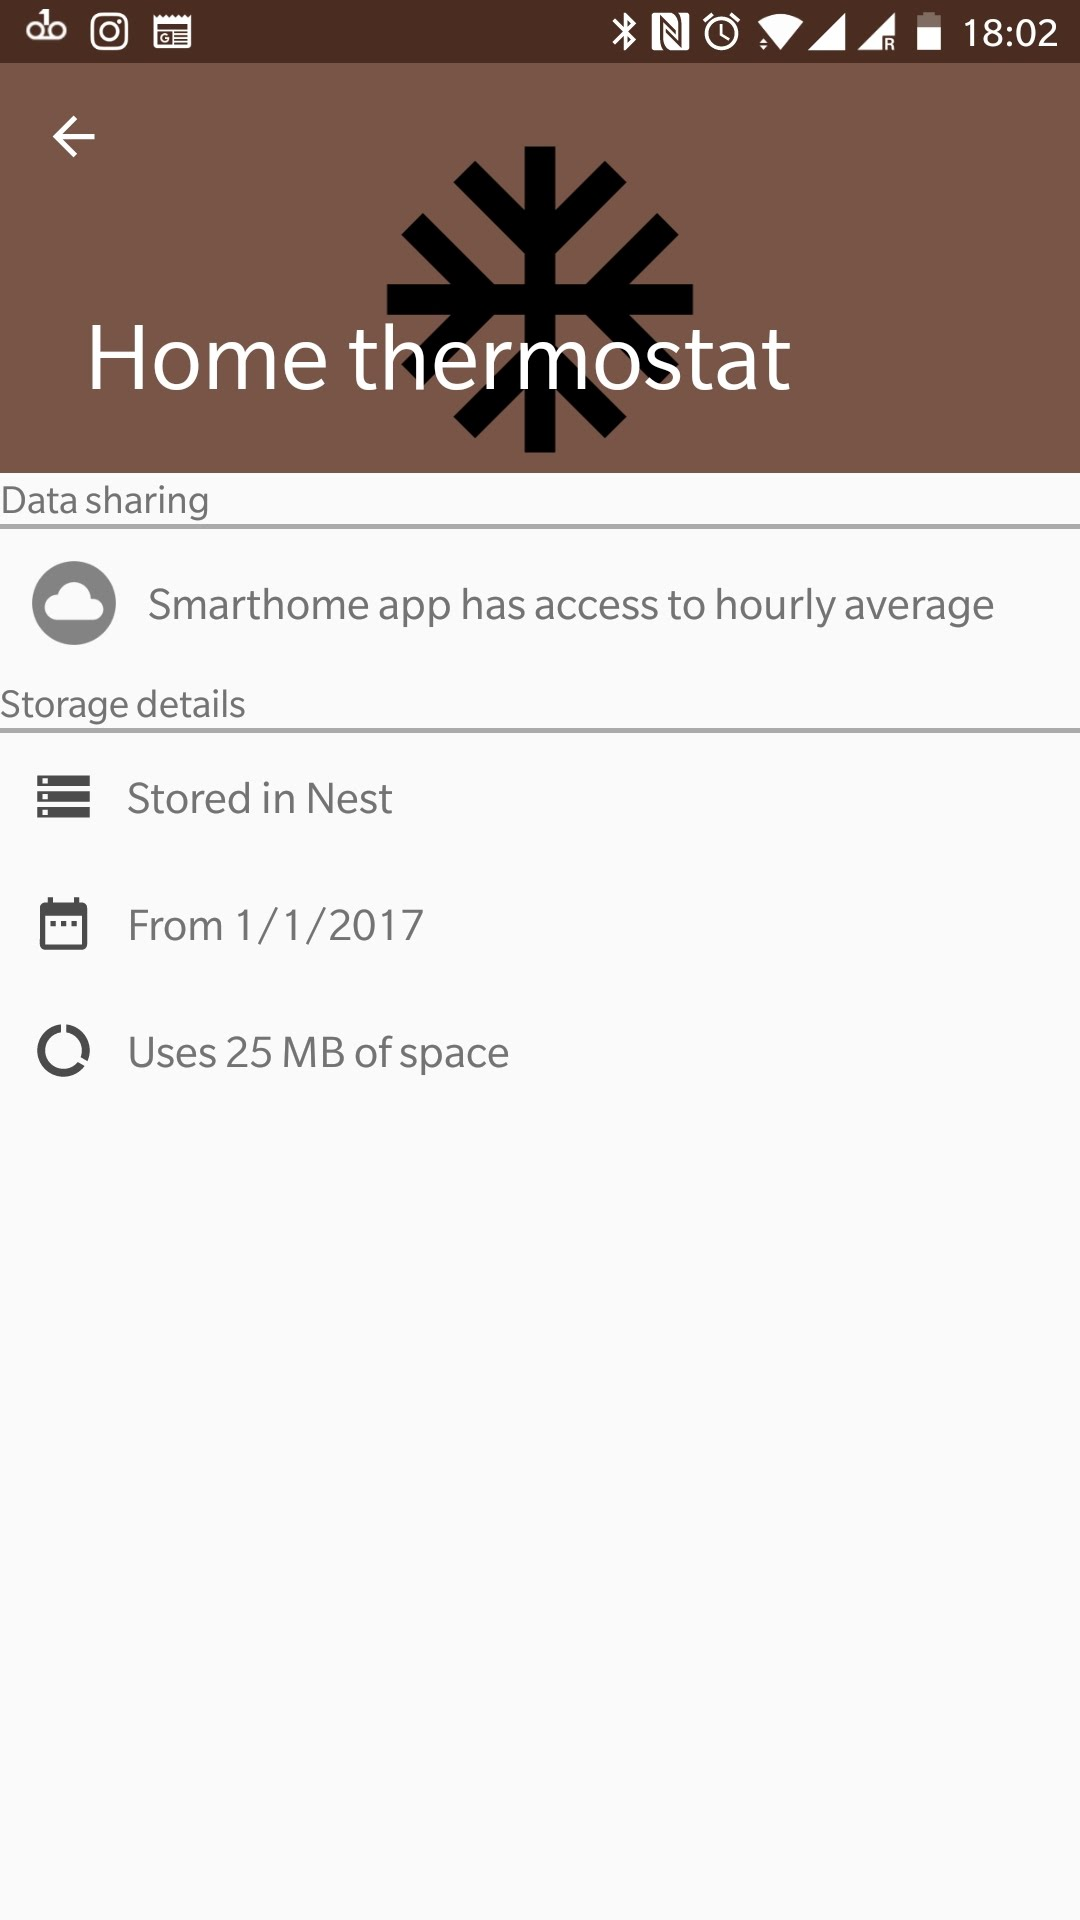
\includegraphics[width=0.95\linewidth]{screen2.jpg}}
	\caption{Details of a particular device}
	\label{fig:screen2}
	\end{subfigure}
	\begin{subfigure}{0.24\textwidth}
	\frame{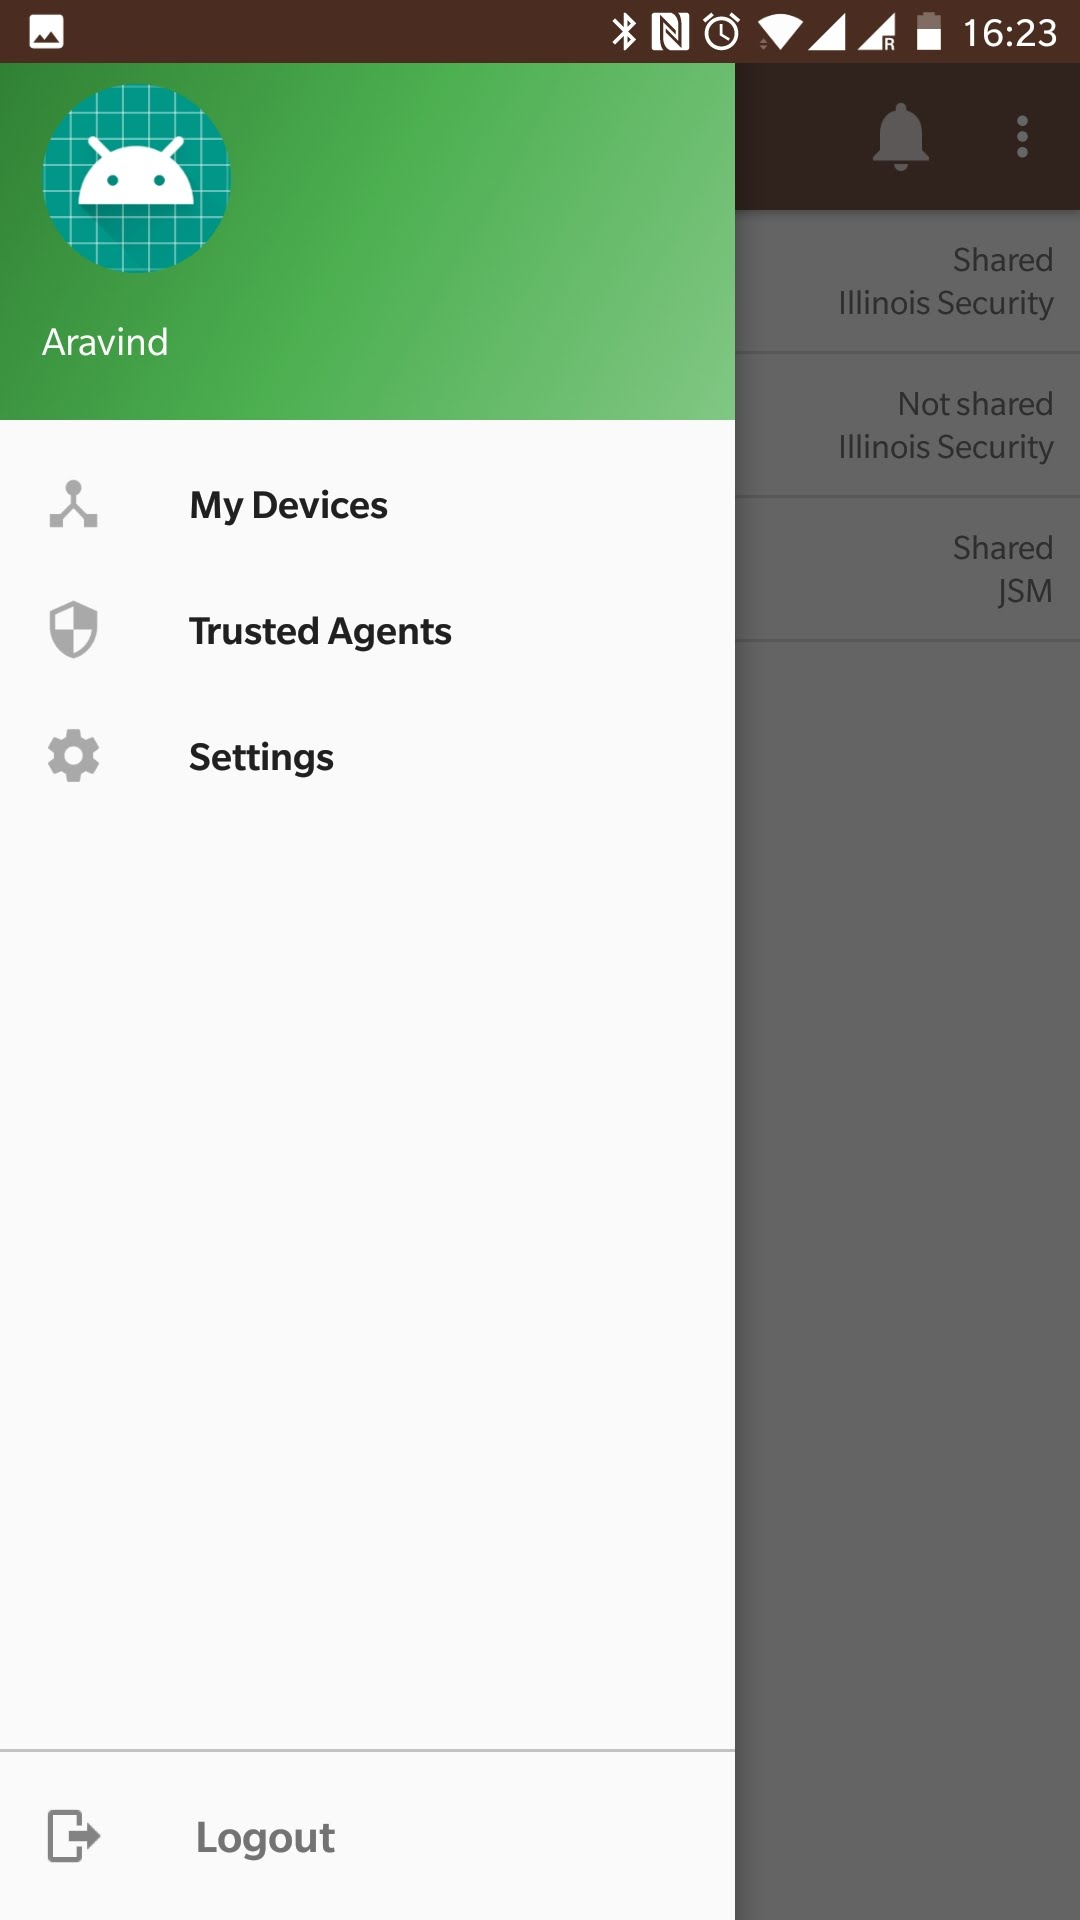
\includegraphics[width=0.95\linewidth]{screen3.jpg}}
	\caption{Navigation drawer}
	\label{fig:screen3}
	\end{subfigure}
	\begin{subfigure}{0.24\textwidth}
	\frame{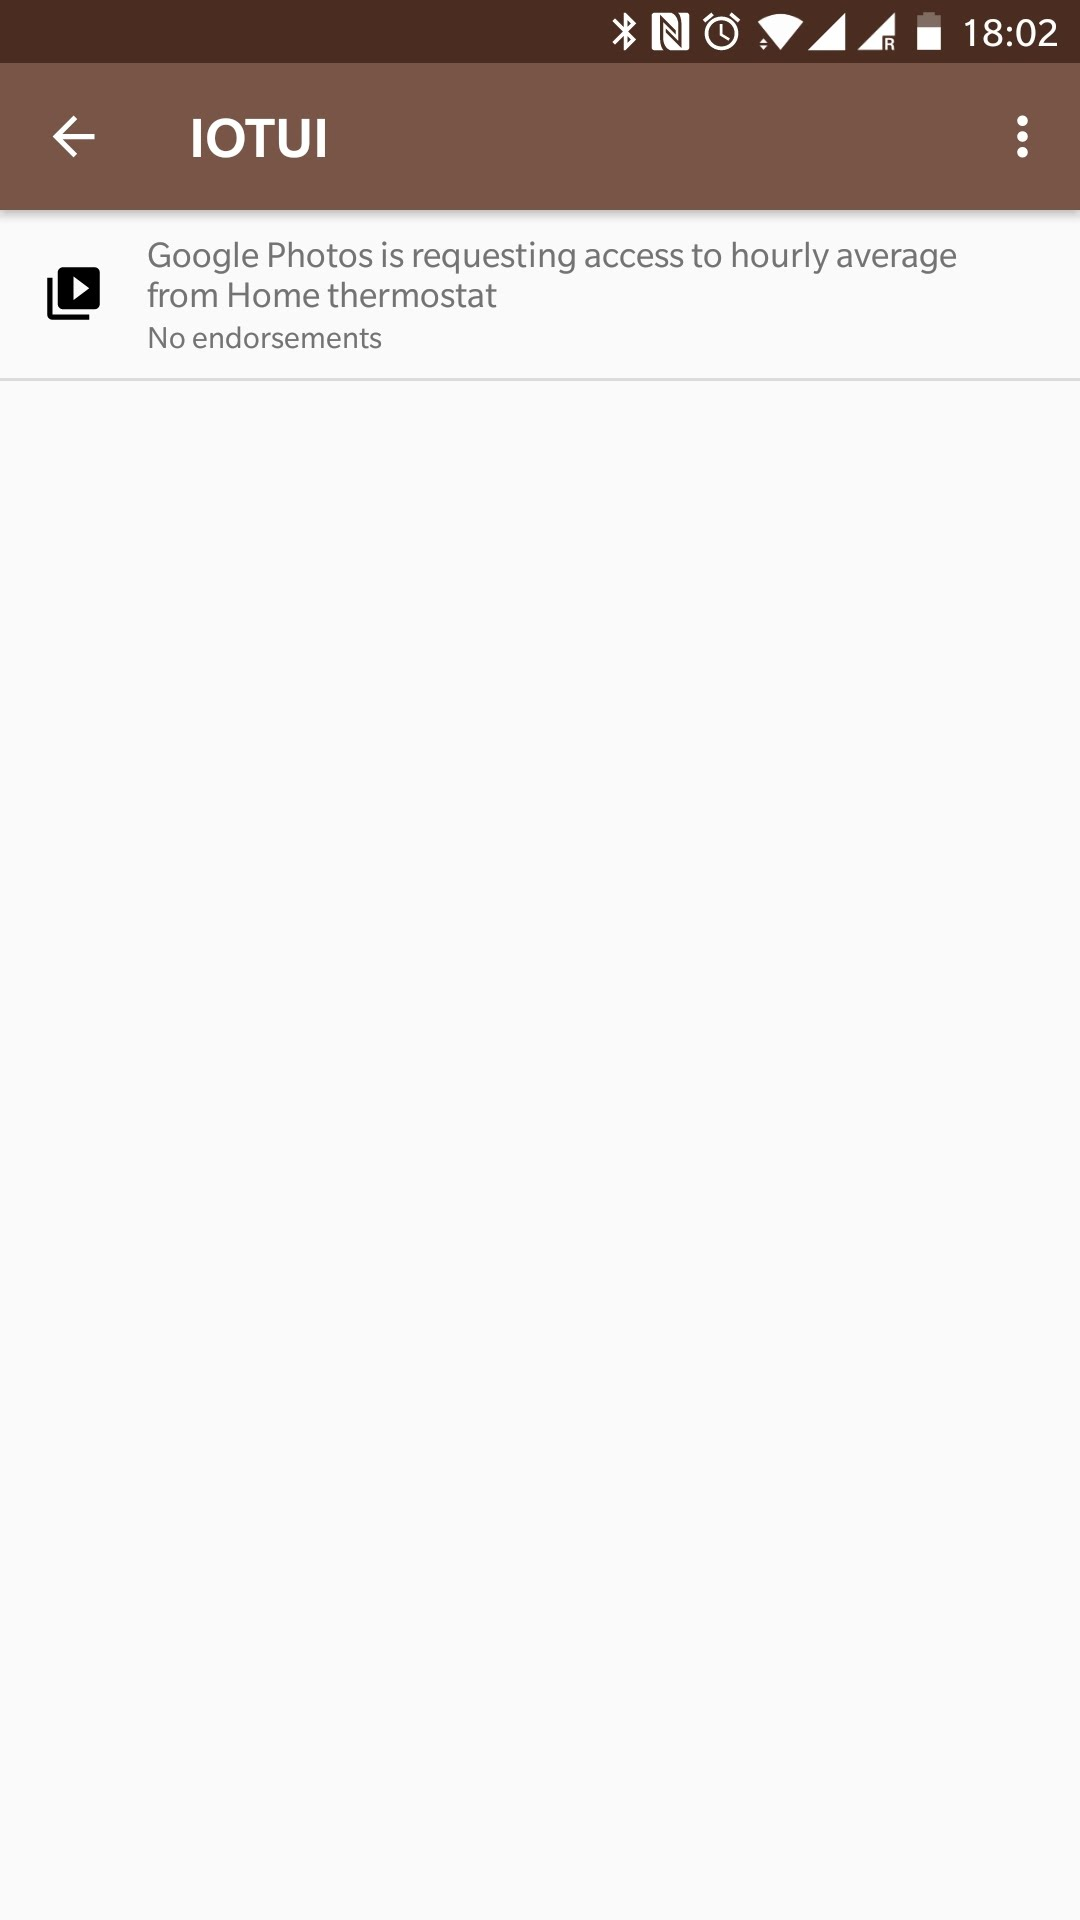
\includegraphics[width=0.95\linewidth]{screen4.jpg}}
	\caption{Notifications screen}
	\label{fig:screen4}
	\end{subfigure}
\caption{UI of the user facing application}\label{fig:screens}
\end{figure*}

\section{Implementation}
The implementation consists of 3 main parts: an Android app, a server manages communications with 3rd parties, and a simulator for Data sources and Data requesters according to the model in~\cite{campbell}. The implementations have been open-sourced under Apache 2.0 licence, and can be found in github:
\begin{itemize}
	\item App: https://github.com/\linebreak[0]aravindsagar/\linebreak[0]cs523-iot-ui-app
	\item Server and simulator: https://github.com/\linebreak[0]ww785612/\linebreak[0]REST\_API\_encryption
\end{itemize}

The repository used for collaborating on the reports: https://github.com/\linebreak[0]aravindsagar/\linebreak[0]cs523-docs

Each component is described in detail below.

\begin{figure}[t]
	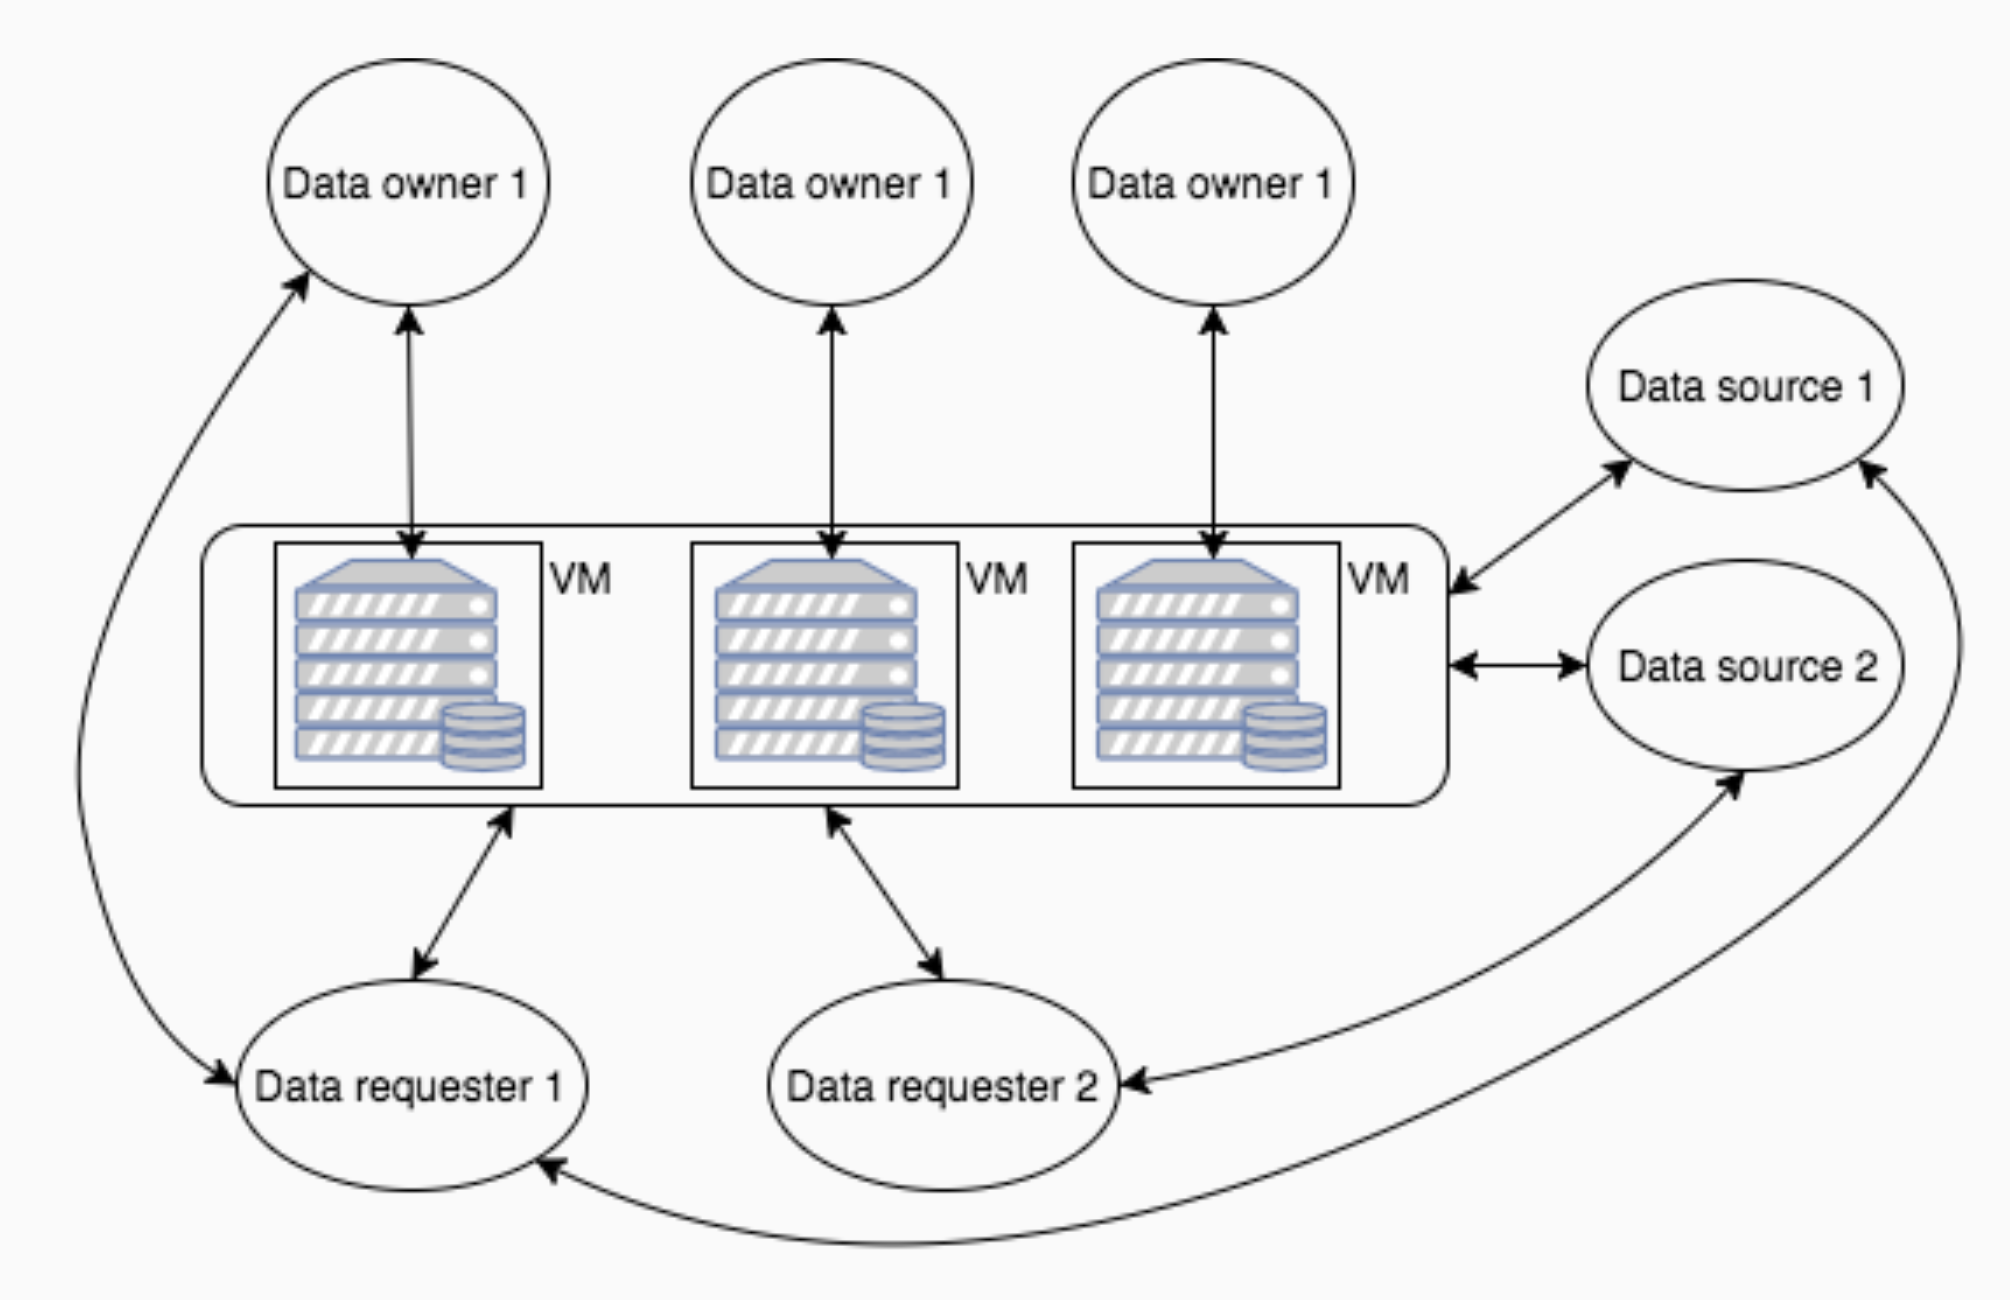
\includegraphics[width=0.95\linewidth]{app_server.png}
	\caption{App-server communication}
	\label{fig:app_server_comm}
\end{figure}
\subsection{Android app}
The component of our solution that a user actually sees and interacts with is an Android app. The reason for going mobile is that mobile devices are now the primary gateway to computing and internet for a vast number of users~\cite{statcount}. Android has emerged as the most popular smartphone OS in recent years~\cite{idc_android}, so we decided to build our application for Android.

The application fulfils all the requirements noted down in the Problem and Solution section. The various screens that enable users to accomplish these functions are shown in Fig.~\ref{fig:screens} (not an exhaustive set). Fig.~\ref{fig:screen1} shows the main entry point into the app. This shows an overview of the various IoT devices owned by the user, and whether the data collected by those devices are shared or not. Clicking on any of these entries shows the details corresponding to that device (Fig.~\ref{fig:screen2}). Users can revoke granted permissions by long pressing an entry in the 'Data sharing' section. Fig.~\ref{fig:screen4} shows the screen which lists the pending data requests. Users can accept or deny each request individually, or accept or reject all requests in one go using the button at bottom-right. Users also have an option to automatically accept/reject all future requests from a particular data requester for a particular device.

The app hides the complexities of collecting data from various sources and communications with the remote server. The basic communication scheme between the app and server is shown in Fig.~\ref{fig:app_server_comm}. The communication happens over https, and the app sends authentication details to the server with each request.

Additionally, the app also stores certain metadata, which is collected by the server by coordinating with data sources and requesters, to present a better description of the third-parties to the user, instead of just using the public key identity of third parties. The various entities in the metadata are defined below:

\begin{enumerate}
	\item Device: This entity represents a physical device owned by the user. The associated details like device name, type, data source used to store data etc. are stored here.

	\item Device data summary: This entity exists because each device can expose various temporal and/or spatial summaries of the data generated by it. It is the responsibility of each device to define its own summaries and make the data source aware of the different summaries. The data requesters are also made aware of the possible summaries so that they can request a suitable level of summarization.

	\item Data source: This entity exists to identify a data source by a name, so that it becomes familiar to the user.

	\item Data requester: Similar to a data source, this entity stores a name for a data requester.

	\item Trusted agent: Similar to a data source, this entity stores a name for a trusted party.

	\item Data access request/permission: Each access request or granted permission must link together a device data summary (the data for which request is being issued/permission is granted), and a data requester.

	\item Endorsement: This keeps track of the endorsements which each data requester has.
\end{enumerate}

The development of the app took place in 3 stages.
\begin{enumerate}
	\item UI mockups and initial user study: We initially created low fidelity mockups of the app screens. This was done by borrowing app design ideas from Material design principles, as well as Rico~\cite{rico}. We then ran a small scale user study where we showed the mockups to a 3 users, explained the tasks that the interface is supposed to accomplish. We then collected their feedbacks on the strengths and weaknesses of the interface.

	The study showed that the following design choices enhance the experience.

	\begin{itemize}
		\item Overall view of the devices and data is very helpful.
		\item Notifications screen is well done because users can see whether the requester is endorsed and act on the notification from the same screen.
		\item Users also feel more comfortable with IoT devices when a privacy-control mechanism like this app is present.
	\end{itemize}

	We also identified some major areas of concern.

	\begin{itemize}
		\item Users need more control over what data is stored. In particular, they might want to delete data between certain time periods.
		\item Users want to minimize the data shared with third parties, and hence each device should expose various spatial and temporal summarizations. 
		\item Guarantee of anonymity is a must when sharing sensitive data with third parties, especially for analytics purposes.
	\end{itemize}

	\item Implementation: The next phase was to develop the actual app, taking into consideration the feedback that we received in the initial phase. Two of the major concerns identified in the previous phase were addressed during the implementation. Firstly, we introduced Device data summaries to make only the bare essential data available to the data requesters. Second, data requesters cannot link collected data to data owner by default. This is a property of the protocol that we are following. However, when the user wants the data requester to provide them personalized services based on the data, they can authorize the data requester to get their public key from the app. We started off the implementation with mock data initially and hooked it up with the server later.

	\item Evaluation of the implemented interface: User evaluation at this stage was done at a larger scale using Amazon mechanical turk. Details can be found in the `User Study' section.
\end{enumerate}
\subsection{Server}
We set up our server on Amazon Web Services EC2. We run a micro-instance with Ubuntu 16.04 to emulate a VM environment provided by a third-party cloud service provider. Our server-side code is written in Python Flask and is supported by Apache2 for HTTP server configuration and MySQL for implementation of the database backend. we used PyCrypto library for encryption/decryption tasks during the Data Management Protocol.

When our Android application communicates with the server, the app must provide credentials (username and password combination) via POST request. This process is processed via HTTPS connection such that app user's credentials are protected against attacks like MITM attacks. On the other hand when Data Sources and Data Requesters interact with our server, they would not require authentication as their messages are protected by cryptographic primitives set up by Hashemi et al. The server is consisted of following interfaces.

\begin{enumerate}
    \item \textbf{/pk}

    Our Android application retrieves Data Owner's public key from the server via this interface. We enforce authentication process to ensure anonymity of Data Owner. Note that Data Owner is allowed to have multiple set of public/private key pairs such that he uses different key for different purposes. This interface provides the default public key (labeled as $K_O$ in Hashemi et al.'s work) to the application.

    \item \textbf{/notify}

    This interface provides information regarding status of data objects and data requests. After authentication, the server makes SQL queries to backend database and dumps the data into JSON format. Then, the query is returned as a return value of the POST request made by the application.

    \item \textbf{/actions}

    Data Owner makes decision on granting/denying data request through this interface. The Android application makes a POST request to this interface with authentication credentials. After verifying identity of the owner, the server validates if the decision made on a request is valid or not. Once this verification has ended, the server processes the action declared by the Data Owner and processes the result to respective Data Requester only when the request is granted. When the request is denied, no further action is performed.

    \item \textbf{/dmp}

    Data Sources and Data Requesters interact with our server via this interface. When message arrives with a POST request, our server first parses the message to label message type for the Data Management Protocol. Note that Data Owner can receive message 1 or 5 from Data Source and message 2 from Data Requester. Accordign to Hashemi et al., The message 2 is transferred via Publisher-Messenger Protocol for the Messaging Service layer. Unfortunately, implementation of Messaging Service is out of scope for this project, so we decided to emulate this service by letting Data Requester directly making requests via HTTP POST request. Incorporating our server with Messaging Service layer is a future work for the project.

    Depending on the type of message, respective cryptographic operations are performed and metadata are parsed from the message. The metadata is written in JSON format, and the server parses the JSON string into SQL query so that a new data object or a new data request is stored into our backend MySQL database.
\end{enumerate}

We assumed our frontend Android application to be honest in our threat model, so our server currently does not have defense against attacks from Application. These attacks include injection attacks via POST request such as SQL injection attacks. Fortifying our server-side implementation against such malicious application is a future work for our project.
\subsection{Data source and requester simulation}
To verify that our system is working properly in the distributed IoT framework~\cite{campbell}, a simulation environment was implemented. This environment simulates the messaging and encryption protocol between data owner and other entities, following the protocol shown in Fig.~\ref{fig:mes_protocol}. Refer to the original paper ~\cite{campbell} for detailed explaination on the protocol in Fig.~\ref{fig:mes_protocol}. Because the main goal of this simulation environment is to verify our implementation on the data-owner side, components that do not directly interact with the data owner are not implemented. 
In the simulation, the data owner hosts a http server on AWS cloud, data requester and data source run on local virtual machines. To transmit information to the data owner, data requester and data source make post requests to the public URL (/dmp) provided by the data owner. All messages are encrypted using the messaging protocol shown in Fig.~\ref{fig:mes_protocol} with some modifications to fit our need. The encryption is done with python library PyCrypto. Because some of the messages are too large to be encrypted or signed using RSA cryptography, we adopted the method of symmetric encryption. In this method, the messages are encrypted using a AES key, the AES key itself is then encrypted using the public key of the data owner and included in the message packet. After the data owner receives the message packet, it uses its private key to decrypt the AES key, and then decrypt the payload of the packet. The message packet also contains a field that labels the message to be one from Fig.~\ref{fig:mes_protocol} so that the data owner knows what information it can expect from this message packet. For more details of the simulation environment, please refer to the source code.


\section{User study}
We conducted a post-implementation user study of our application, with the intention of answering 2 main questions.
\begin{enumerate}
	\item Does the application communicate well with the user? That is, can a user easily understand the information laid out by the app?
	\item Does the privacy enhancing measures like data summarization really make a difference in users' decision to share data with third parties?
\end{enumerate}

\subsection{User study setup}

\textit{Survey questions}: The survey involved presenting the users with screenshots of the application, and collecting their reponses to determine whether the app meets its goals. To measure how well users understand the information presented in the app, we asked the following questions:
\begin{enumerate}
	\item Who stores the data generated by the home thermostat?
	\item Who is requesting access to hourly averages of the thermostat data?
\end{enumerate}

These additional questions were asked to ascertain conditions under which users are more willing to share their data with third parties.
\begin{enumerate}
	\item In the given example, the data requester is asking only for hourly averages of your thermostat data, and not the entire data collected by the device. Does this make you more willing to share the data?
	\item If a third party data requester has endorsements from entities known to you, will you be more willing to share your data with them?
\end{enumerate}

\textit{Test platform}: To gain feedback about the app from a wide audience, we used Amazon mechanical turk for conducting the study~\cite{mturk}. We created a survey in the platform using app screenshots and the questions listed above. We offered \$0.15 for each participant and collected responses of 100 participants over the course of a few hours.

\subsection{User study results}
A summary of the responses by the users is shown in Fig.~\ref{fig:user_study}. The data shows that almost 70\% of the users were aware of the source of their data. More importantly, 90\% of the users correctly identified the data requester. Around 50\% of the users were more willing to share their data in case of endorsements or data summarizations. This shows that users do care about privacy and third-party trust mechanisms. Incorporating such features will be essential to collect data from maximum number of users in an IoT system.

\section{Challenges and future work}
There exists several challenges to implement our solution. We would to address these challenges in this section. 

\begin{enumerate}
\item \textbf{Simulating Roles}

Since our work is based on a theoretical model, we need to simulate each entity. During this simulation process, we may run into some implementation problems regarding details that are not explained in the literature. Thus, we need to make assumptions and augment the model in order to proceed our project. Furthermore, we may not have accurate performance benchmarks for our evaluation as we work on a simulated environment for testing our framework. 

\item \textbf{Designing User Interface}

Effective application design is an active area of research. Designing our front-end application would be the most challenging task for our project. We would like to explore Deka et al.'s~\cite{rico} large repository of mobile app design to achieve our goal for the project. Davies et al.~\cite{davies} discusses key challenges and concerns regarding how to design user policies that mediate between user and application. While they do not directly provide a clear-cut solution to the problem, authors provide a list of possible approaches to improve effectiveness of user policies.  

\item \textbf{User Study for App Interface}

The challenges related to conducting a user research for the mobile app are two fold.

First, we are building an interface for which the backend is unfamiliar, and not available yet. This means that users need to know more background information about the interface for which we seek feedback. In particular, most of the IoT systems that exist now are centralized, and provides coarse-grained permissioning. By contrast, the system that we are targeting is distributed, user-centric, and fine grained in terms of third party data access permissions. Users need to know this to provide effective feedback about the interface.

Second, IoT is still in its infancy, and it's hard to find enthusiast users of IoT devices. We overcome this by treating smartphone sensors as basic IoT devices and building a story for user interaction with the application in terms of sensor data available from smartphones.
\end{enumerate}

\section{Conclusion}
We present a User-Friendly IoT Data Management Framework based on Hashimi et al.'s IoT Data sharing model. We successfully implemented our solution and deployed our framework on a Android application and a VM hosted by Amazon EC2 cloud. We simulated the Data Management Protocol proposed by Hashimi et al. and successfully interacted with Data Sources and Data Requesters. Our User Study shows that our solution effectively provided summarized information to end-users to assist their decision making procedures for each data request. While our solution builds on a theoretical data sharing model, we believe our solution provides a useful insight to solving future IoT data sharing problems.

\begin{thebibliography}{00}
\bibitem{davies} Davies, Nigel, et al. ``Privacy mediators: Helping iot cross the chasm.'' Proceedings of the 17th International Workshop on Mobile Computing Systems and Applications. ACM, 2016.
\bibitem{campbell} Hashemi, Sayed Hadi, et al. ``World of Empowered IoT Users.'' Internet-of-Things Design and Implementation (IoTDI), 2016 IEEE First International Conference on. IEEE, 2016.
\bibitem{zhang} Zhang, Nan, et al. ``Understanding IoT Security Through the Data Crystal Ball: Where We Are Now and Where We Are Going to Be.'' arXiv preprint arXiv:1703.09809. arXiv, 2017
\bibitem{statcount} (2016, Nov.) ``Mobile and tablet internet usage exceeds desktop for first time worldwide.'' Statcounter global stats. [Online]. Available: http://gs.statcounter.com/press/mobile-and-tablet-internet-usage-exceeds-desktop-for-first-time-worldwide (Accessed Oct 24, 2017)
\bibitem{tz} Ahmed M. Azab, et al. 2014. ``Hypervision Across Worlds: Real-time Kernel Protection from the ARM TrustZone Secure World.'' In Proceedings of the 2014 ACM SIGSAC Conference on Computer and Communications Security (CCS '14). ACM, New York, NY, USA, 90-102. DOI: http://dx.doi.org/10.1145/2660267.2660350
\bibitem{leaky} Wang, Wenhao, et al. ``Leaky Cauldron on the Dark Land: Understanding Memory Side-Channel Hazards in SGX.'' ACM Computer and Communications Security (CCS ’17), October, 2017.
\bibitem{mengjia} Yan, Mengjia, et al. 2017. ``Secure Hierarchy-Aware Cache Replacement Policy (SHARP): Defending Against Cache-Based Side Channel Atacks.'' In Proceedings of the 44th Annual International Symposium on Computer Architecture (ISCA '17). ACM, New York, NY, USA, 347-360. DOI: https://doi.org/10.1145/3079856.3080222
\bibitem{raccoon} Rane, Ashay, et al. ``Raccoon: Closing digital side-channels through obfuscated execution.'' In USENIX Security Symposium (2015).
\bibitem{atzori} Atzori, Luigi, Antonio Iera, and Giacomo Morabito. ``The internet of things: A survey." Computer networks 54.15 (2010): 2787-2805.
\bibitem{itu} (2012, Jun) ``Overview of Internet of Things.'' ITU-T Recommendations. Available: http://www.itu.int/ITU-T/recommendations/rec.aspx?rec=y.2060 (Accessed Oct 25, 2017)
\bibitem{idc} (2015, Jun) ``Internet of Things Market to Reach \$1.7 Trillion by 2020''. The Wall Street Journal. Available: https://blogs.wsj.com/cio/2015/06/02/internet-of-things-market-to-reach-1-7-trillion-by-2020-idc/ (Accessed Oct 25, 2017)

\end{thebibliography}

\end{document}